\documentclass[10pt, a4paper]{article}

\usepackage[margin=0.75in]{geometry}
\usepackage{graphicx}
\usepackage{booktabs}
\usepackage{array}
\usepackage{xcolor}
\usepackage{hyperref}
\usepackage{caption}
\usepackage{enumitem}
\usepackage{fancyhdr}
\usepackage{titlesec}
\usepackage[utf8]{inputenc}
\usepackage[T1]{fontenc}
\usepackage{lmodern}
\usepackage{amsmath}
\usepackage{float}

% Brand colors
\definecolor{argosNavy}{HTML}{0d1b2a}
\definecolor{argosTeal}{HTML}{00b4d8}
\definecolor{argosGreen}{HTML}{4caf50}
\definecolor{argosCoral}{HTML}{e06c75}
\definecolor{argosGold}{HTML}{ffd54f}
\definecolor{argosGray}{HTML}{555555}

\hypersetup{colorlinks=true, linkcolor=argosTeal, urlcolor=argosTeal}

\titleformat{\section}{\large\bfseries\color{argosNavy}}{\thesection}{0.7em}{}
\titlespacing*{\section}{0pt}{0.6em}{0.3em}
\titleformat{\subsection}{\normalsize\bfseries\color{argosNavy}}{\thesubsection}{0.6em}{}
\titlespacing*{\subsection}{0pt}{0.4em}{0.2em}

\pagestyle{fancy}
\fancyhf{}
\rhead{\textcolor{argosGray}{\small Confidence Brief -- 1,497-segment B3}}
\lhead{\textcolor{argosGray}{\small Argos VSP-LLM}}
\rfoot{\thepage}
\renewcommand{\headrulewidth}{0.4pt}

\setlength{\parskip}{0.35em}
\setlength{\parindent}{0pt}
\captionsetup{font=small,skip=2pt}

\graphicspath{{../../presentation_materials_20260224/01_plots_for_slides/}}

\title{
  \vspace{-1.6cm}
  \textbf{Confidence Sidecar: 5-Page Brief}\\
  \normalsize\textcolor{argosGray}{1,497-segment B3 decode -- the operational story}
}
\author{}
\date{}

\begin{document}
\maketitle
\thispagestyle{fancy}
\vspace{-2cm}

\noindent\fcolorbox{argosGray}{argosGray!10}{%
\begin{minipage}{0.97\textwidth}
\small\textbf{Source.} Per-token confidence sidecar from the 1,497-segment B3 decode (\texttt{/tmp/vsp\_b3\_1497\_out/confidence-172610.json}), joined with baseline ground truth (IS, WER, NEA F1). 23,261 hyp words. Hypotheses are bit-identical to the baseline decode -- the 59.17\% pooled vs 64.05\% mean-of-segment WER gap is purely the pooled-vs-averaged divergence on a heavy-tailed distribution.

\textbf{Scope of this brief.} This document summarises the deployment-relevant findings of the full confidence analysis: how strongly confidence predicts quality, where to set the gate, what slips through, and the failure-mode taxonomy. \emph{Per-word band calibration is not covered here} -- see the comprehensive 17-page report for the calibration analysis (overall ECE, stratified band reliability, and the three-tier display policy).
\end{minipage}}

% ===================================================================
\section*{Headline findings}
% ===================================================================

\textbf{TL;DR.} The average per-word confidence inside a segment (mean of the model's max-softmax probabilities, one per output word) predicts the segment's overall quality with Pearson $r = +0.84$ against the Intelligibility Score. That single number is enough to filter bad outputs out at runtime. The remaining failures break into a small set of categories that need beam-aggregation or topic context to detect.

\textbf{Term key.} \textbf{IS} = Intelligibility Score (0--5, mean = 2.52). \textbf{NIV-Y} = ``clearly intelligible'' (IS $\ge 3.80$). \textbf{NIV-N} = ``not intelligible'' (IS $< 2.0$). \textbf{mean\_word\_prob} = per-segment average of per-word probs (each per-word prob = min over its sub-tokens). \textbf{WER / WWER} = word error rate / weighted WER (content tokens count $2\times$).

\begin{enumerate}[leftmargin=*, itemsep=2pt, topsep=2pt]
  \item \textbf{Mean word probability is the single best confidence aggregate} -- Pearson $r = +0.837$ with IS, $-0.714$ with WER, $-0.749$ with WWER ($n = 1{,}427$). Geomean prob, mean entropy, mean margin, and \texttt{frac\_p\_ge\_0.85} all sit within $\sim 0.03$ $r$ of this -- different shadows of the same signal.
  \item \textbf{Confidence is a strong segment-level filter} -- AUC $= 0.917$ for NIV-N, $0.921$ for NIV-Y from \texttt{mean\_prob} alone. At \texttt{mean\_word\_prob} $\ge 0.80$ we keep $\mathbf{78\%}$ of NIV-Y and admit only $\mathbf{9}$ NIV-N out of 405 trusted segments (2.2\% false-trust). For zero-tolerance use, add \texttt{duration $\ge 1.5$s AND mean\_entropy $\le 0.7$} $\to$ zero false-bads at $\sim 30\%$ recall.
  \item \textbf{Hallucinations mostly self-flag} -- of 223 fluent-but-wrong segments, only \textbf{3} (1.3\%) have \texttt{mean\_prob} $\ge 0.85$. Median \texttt{mean\_prob} 0.541 vs 0.759 healthy; entropy AUC ties with prob AUC. The literature's worst-case ``fluent fabrications at $p > 0.95$'' failure mode is rare in this data.
  \item \textbf{Different failure modes need different signals} -- 503 IS$<$2 segments classify as Wrong Topic 68\%, Hallucination 10\%, Right Topic Wrong Details 15\%, Signal Loss 0.2\%, Accumulated Errors 7\%. Hallucination + Signal Loss ($\approx$10\%) are catchable from confidence + length-ratio. The remaining $\sim$90\% require the reference (semantic / NEA) or a runtime substitute -- \textbf{Mission 6} (all-20-beams) and \textbf{Mission 8} (topic-LM) are the next-sprint priorities.
\end{enumerate}

% ===================================================================
\section{What confidence is, and what it predicts}
% ===================================================================

\begin{figure}[H]
\centering
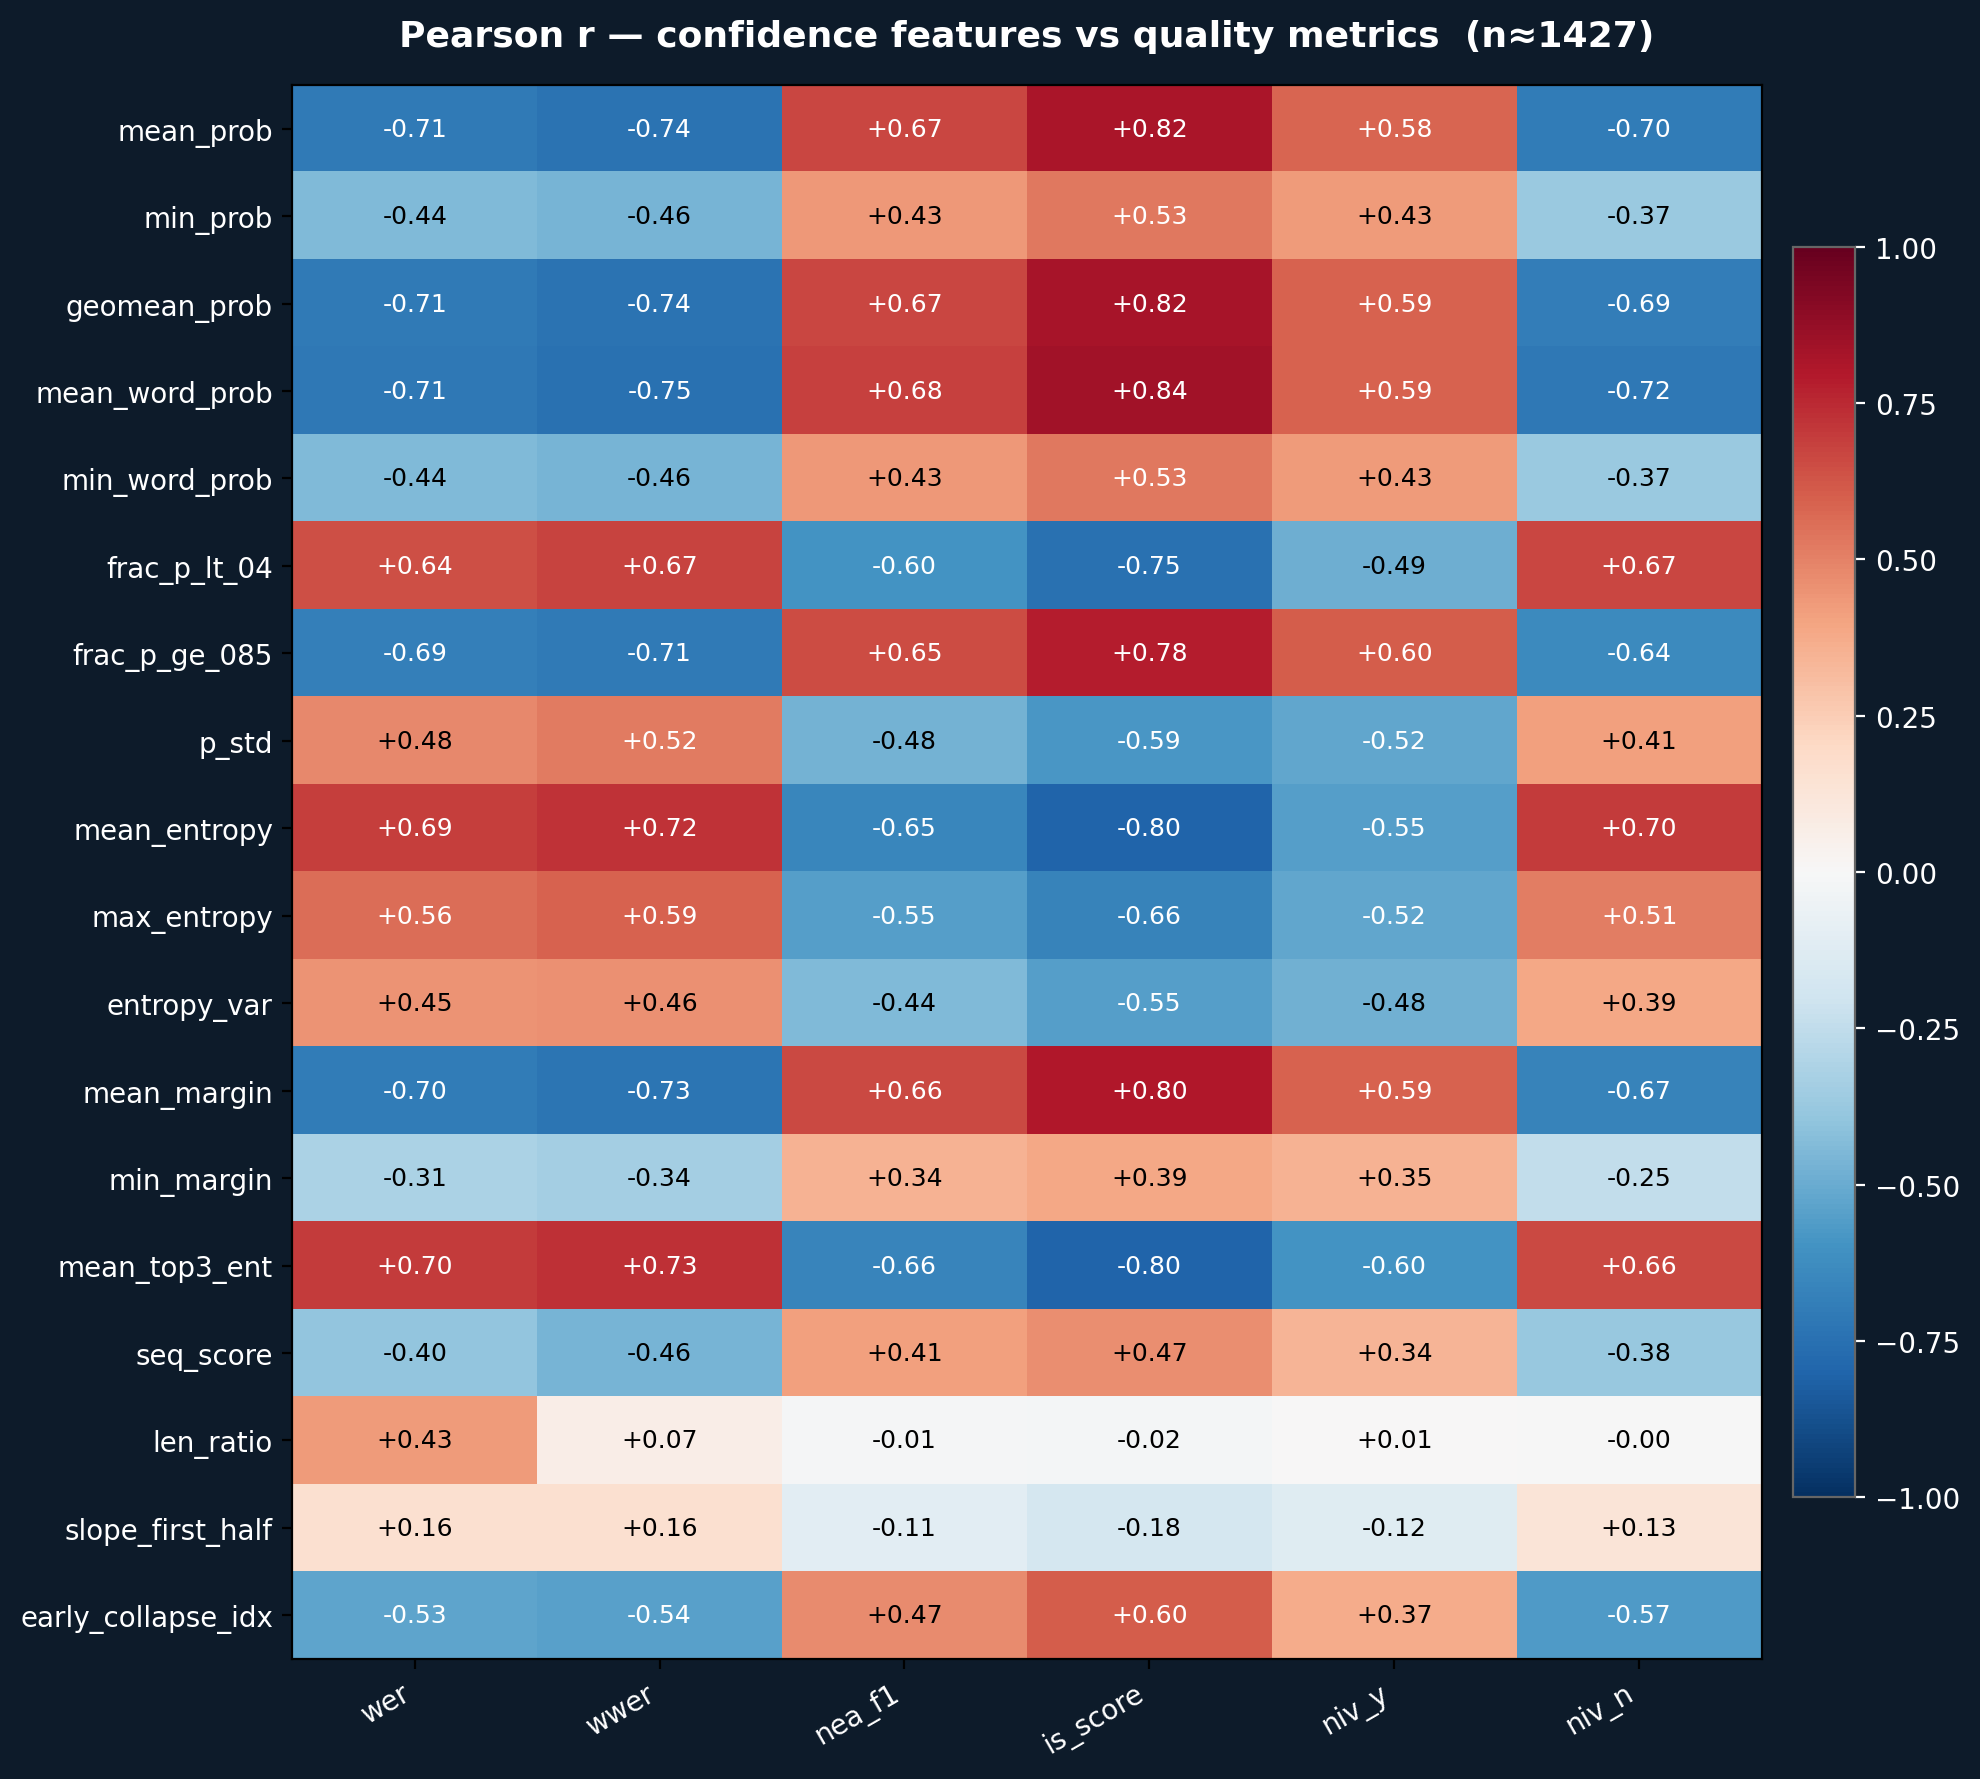
\includegraphics[width=0.92\textwidth]{conf_correlation_heatmap.png}
\caption{Pearson correlation matrix. Rows: confidence-derived features. Columns: quality metrics. Mean-aggregates of probability, entropy, margin, and ``green-band-fraction'' all hit $|r| \ge 0.7$ against IS / WER / WWER -- they're interchangeable as quality signals. \texttt{min\_word\_prob} is meaningfully weaker (one bad word can occur in an otherwise-fine segment). Spearman $\rho$ tracks Pearson $r$ within $0.06$ for confidence-vs-IS pairs, so the relationship is not a linearity artifact.}
\end{figure}

\textbf{Top-5 features by} $|r|$ \textbf{with IS:} \texttt{mean\_word\_prob} $+0.837$, \texttt{geomean\_prob} $+0.822$, \texttt{mean\_prob} $+0.818$, \texttt{mean\_entropy} $-0.804$, \texttt{mean\_margin} $+0.803$. Three of the four leading signals explain $\sim 65\%$ of IS variance with a single linear term. Top-3-only entropy is $r = +0.946$ redundant with full-distribution entropy -- the cheap version isn't enough; genuine beam-level information needs all 20 hypotheses (Mission 6).

\textbf{Practical reading.} For runtime quality estimation we don't need anything fancier than averaging the per-word probabilities the model already produces.

% ===================================================================
\section{Filtering: operating points and what slips through}
% ===================================================================

\begin{figure}[H]
\centering
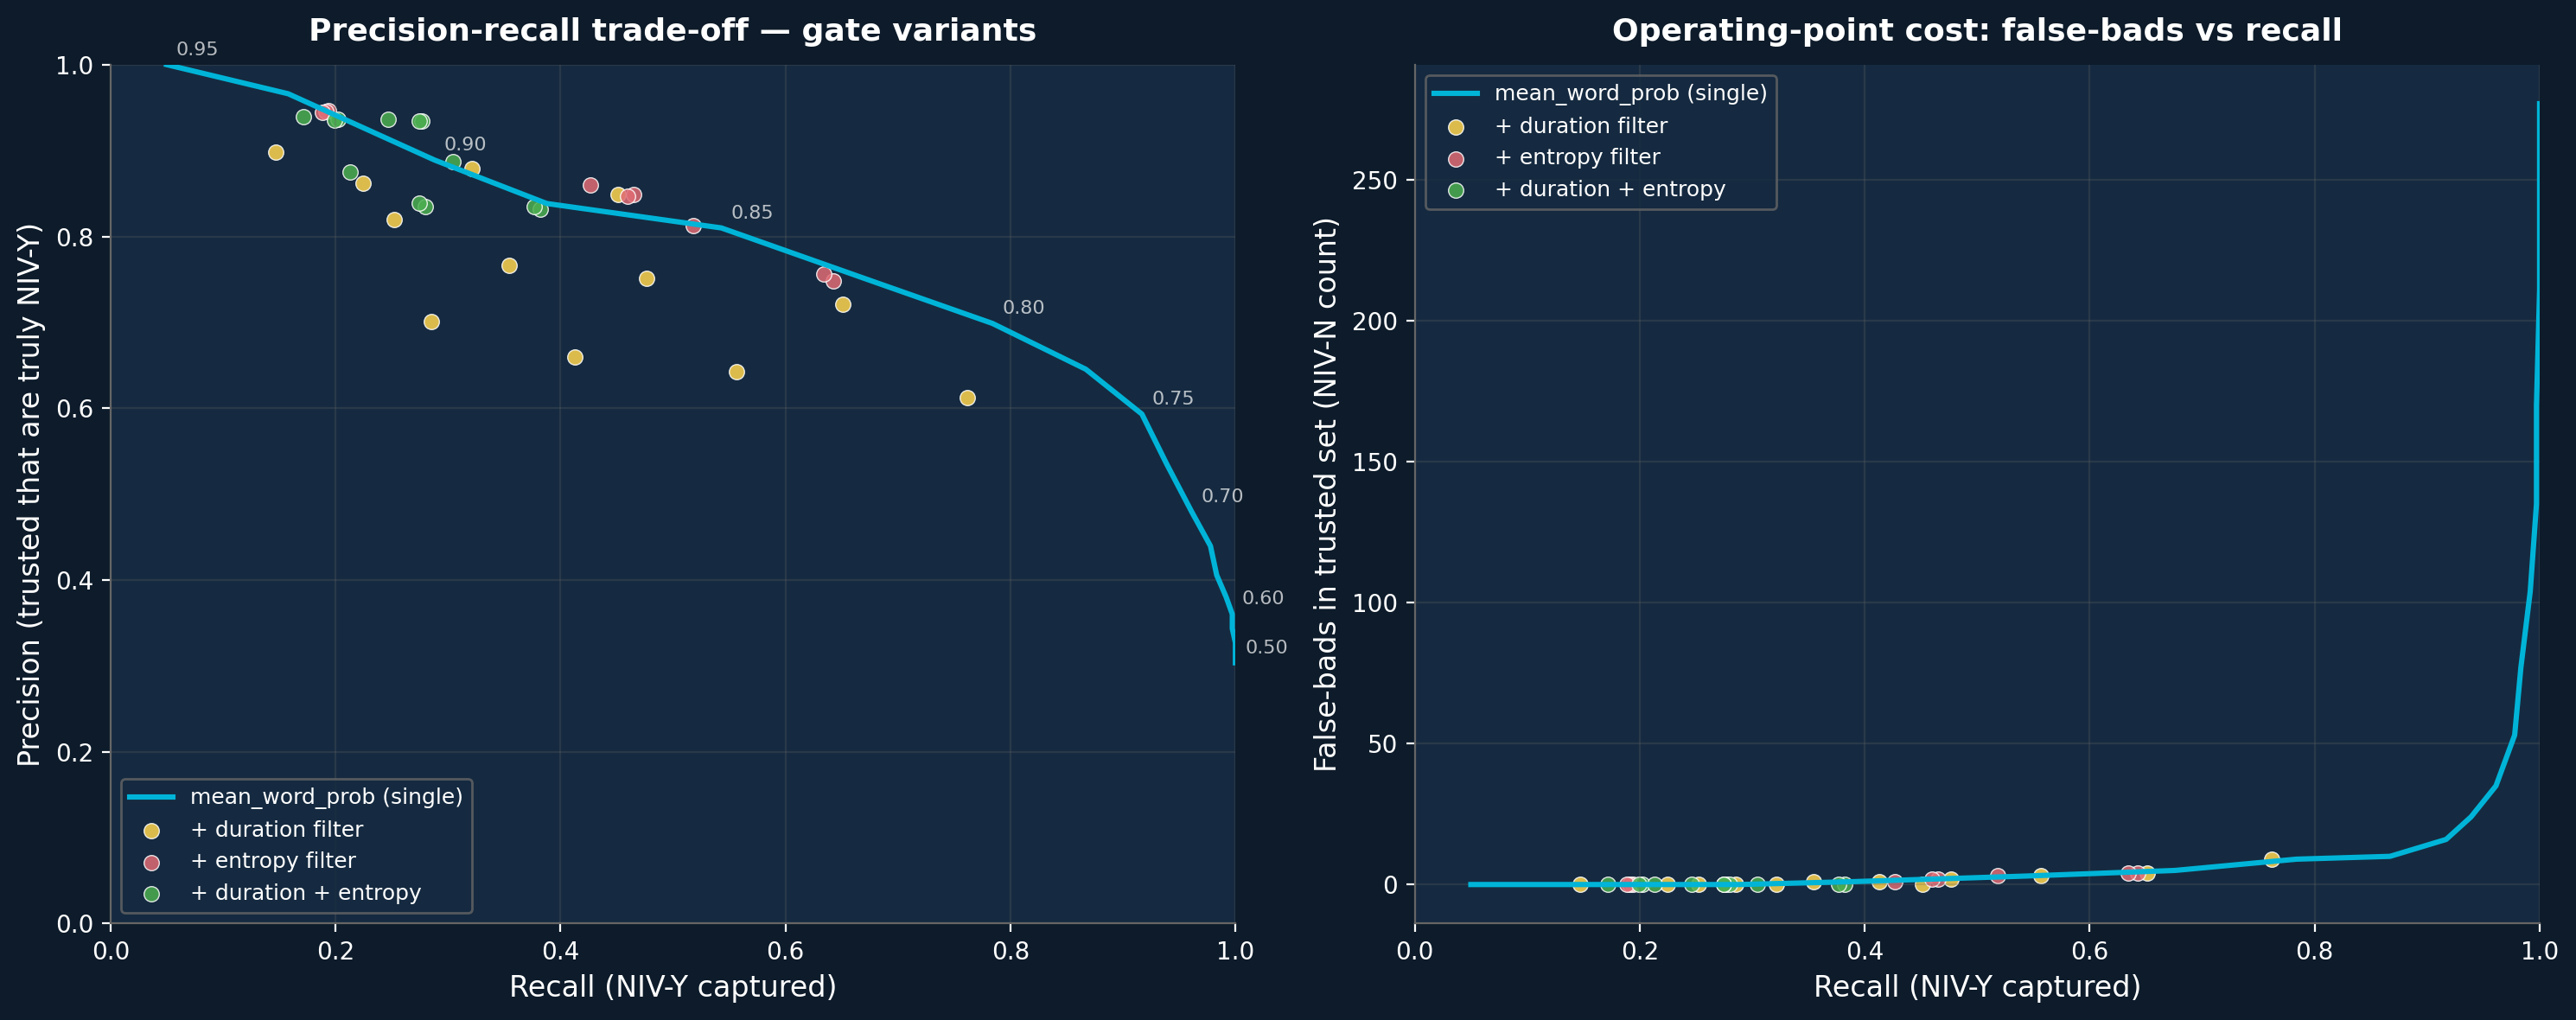
\includegraphics[width=0.95\textwidth]{conf_operating_points.png}
\caption{Left: precision-recall trade-off. Cyan curve sweeps \texttt{mean\_word\_prob} alone; coloured dots overlay duration / entropy / triple-signal gates. Right: false-bad count (NIV-N inside trusted set) as recall grows. Adding constraints trades recall faster than it adds precision, but enables zero-false-bad operating points for high-stakes use.}
\end{figure}

\begin{table}[H]
\centering
\small
\begin{tabular}{lp{0.36\textwidth}rrrr}
\toprule
\textbf{Operating point} & \textbf{Gate} & \textbf{Prec.} & \textbf{Recall} & \textbf{False-bads} & \textbf{Vol.\,\%} \\
\midrule
Loose (high recall)    & \texttt{mwp $\ge 0.75$}                                          & 59.3\% & 91.7\% & 16 & 39.1\% \\
\textbf{Balanced}      & \texttt{mwp $\ge 0.80$}                                          & \textbf{69.9\%} & \textbf{78.4\%} & 9  & 28.4\% \\
Strict precision       & \texttt{mwp $\ge 0.85$}                                          & 81.0\% & 54.3\% & 3  & 17.0\% \\
$+$ duration filter    & \texttt{mwp $\ge 0.85$ AND dur $\ge 1.5$s}                       & 87.9\% & 32.1\% & 0  & 9.3\%  \\
\textbf{Zero-false-bad} & \texttt{mwp $\ge 0.85$ AND dur $\ge 1.5$s AND ent $\le 0.7$}    & \textbf{88.7\%} & \textbf{30.5\%} & \textbf{0}  & 8.7\%  \\
\bottomrule
\end{tabular}
\end{table}

\subsection{Who slips through? False-good profile}

\begin{figure}[H]
\centering
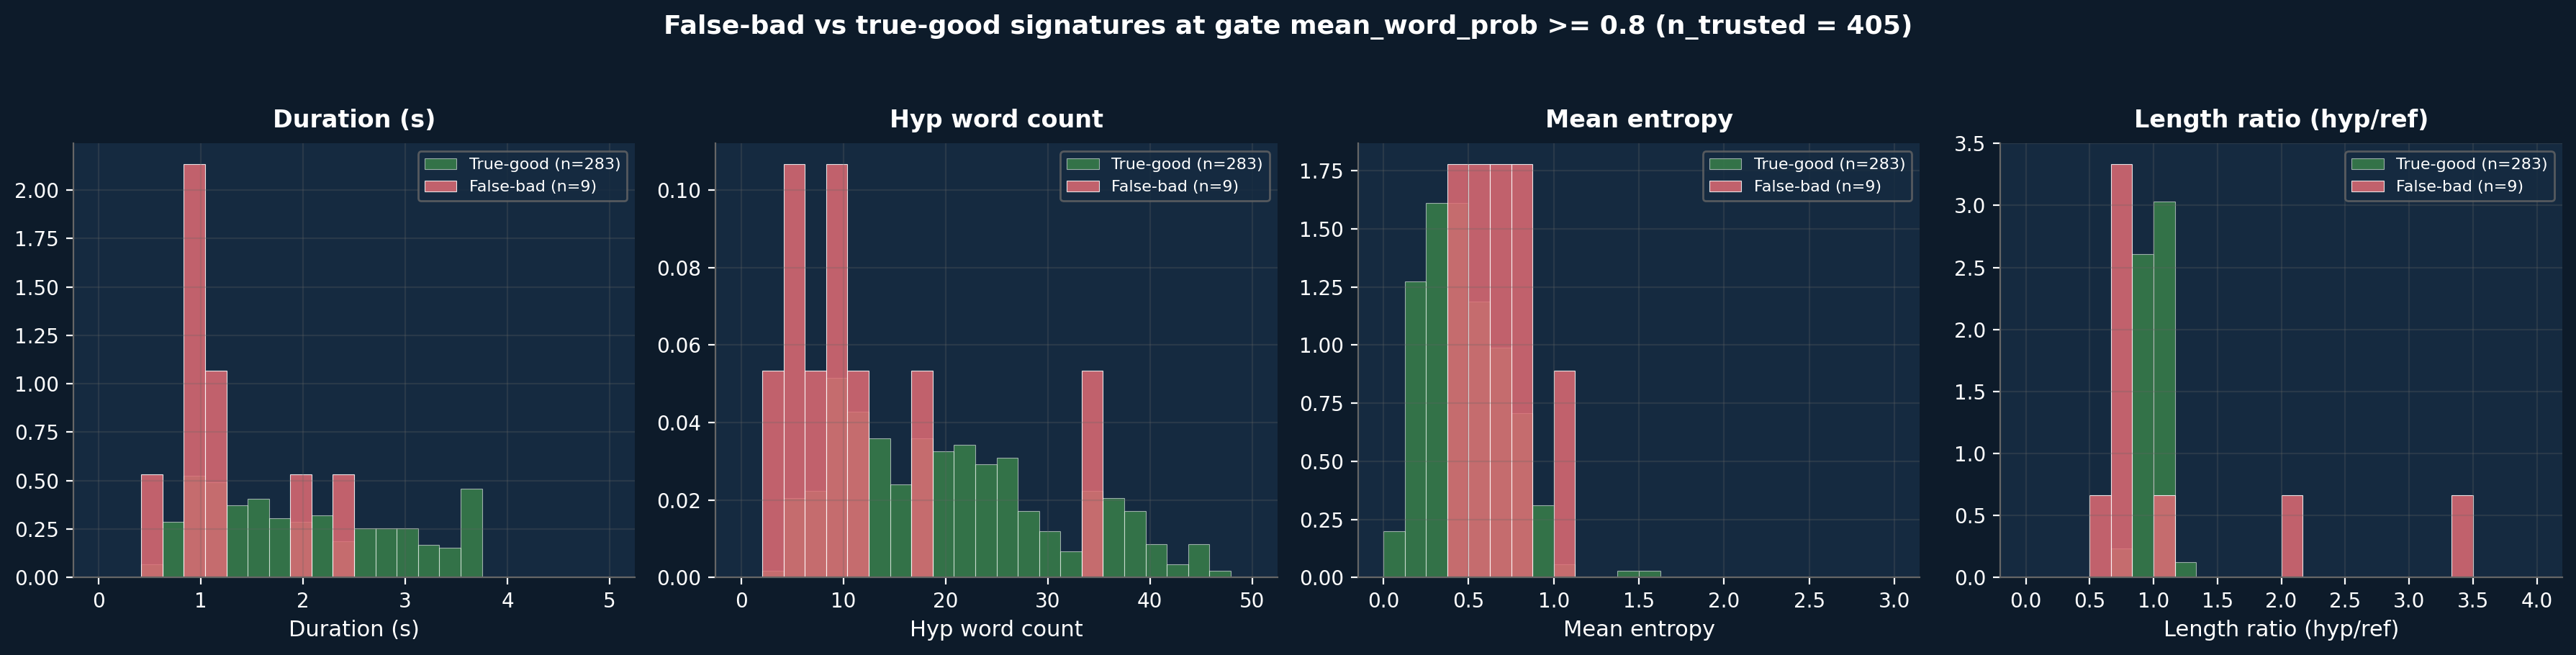
\includegraphics[width=0.95\textwidth]{conf_false_good_signatures.png}
\caption{Density of true-good (green) vs false-bad (coral) at \texttt{mean\_word\_prob} $\ge 0.80$. \textbf{The smoking gun: false-bads are systematically SHORT.} Median duration 0.98s vs 1.86s; median hyp word count 9 vs 19; mean entropy is $+0.20$ higher.}
\end{figure}

False-bads are systematically segments where the model has too little material to constrain its output -- short clips with a handful of words give the language prior room to commit to a fluent-but-wrong answer. \textbf{Visual cues:} segment duration is a free runtime proxy for visual quality. A real visual quality model (lip occlusion, face-frame coverage, head pose) would catch more, but is out-of-pipeline today. \textbf{Topic context:} a surrounding-sentence LM conditioned on the source video's topic could rescore the hyp and flag drift; out-of-pipeline today. \textbf{Beam disagreement} (Mission 6) is the most tractable next-sprint signal for the truly fluent-and-plausible cases that confidence alone cannot detect.

% ===================================================================
\section{Failure modes in confidence space}
% ===================================================================

The 503 IS$<$2 segments classify into five mutually-exclusive categories (March 2026 deck taxonomy, evaluated $1 \to 5$). Each segment gets exactly one label.

\begin{figure}[H]
\centering
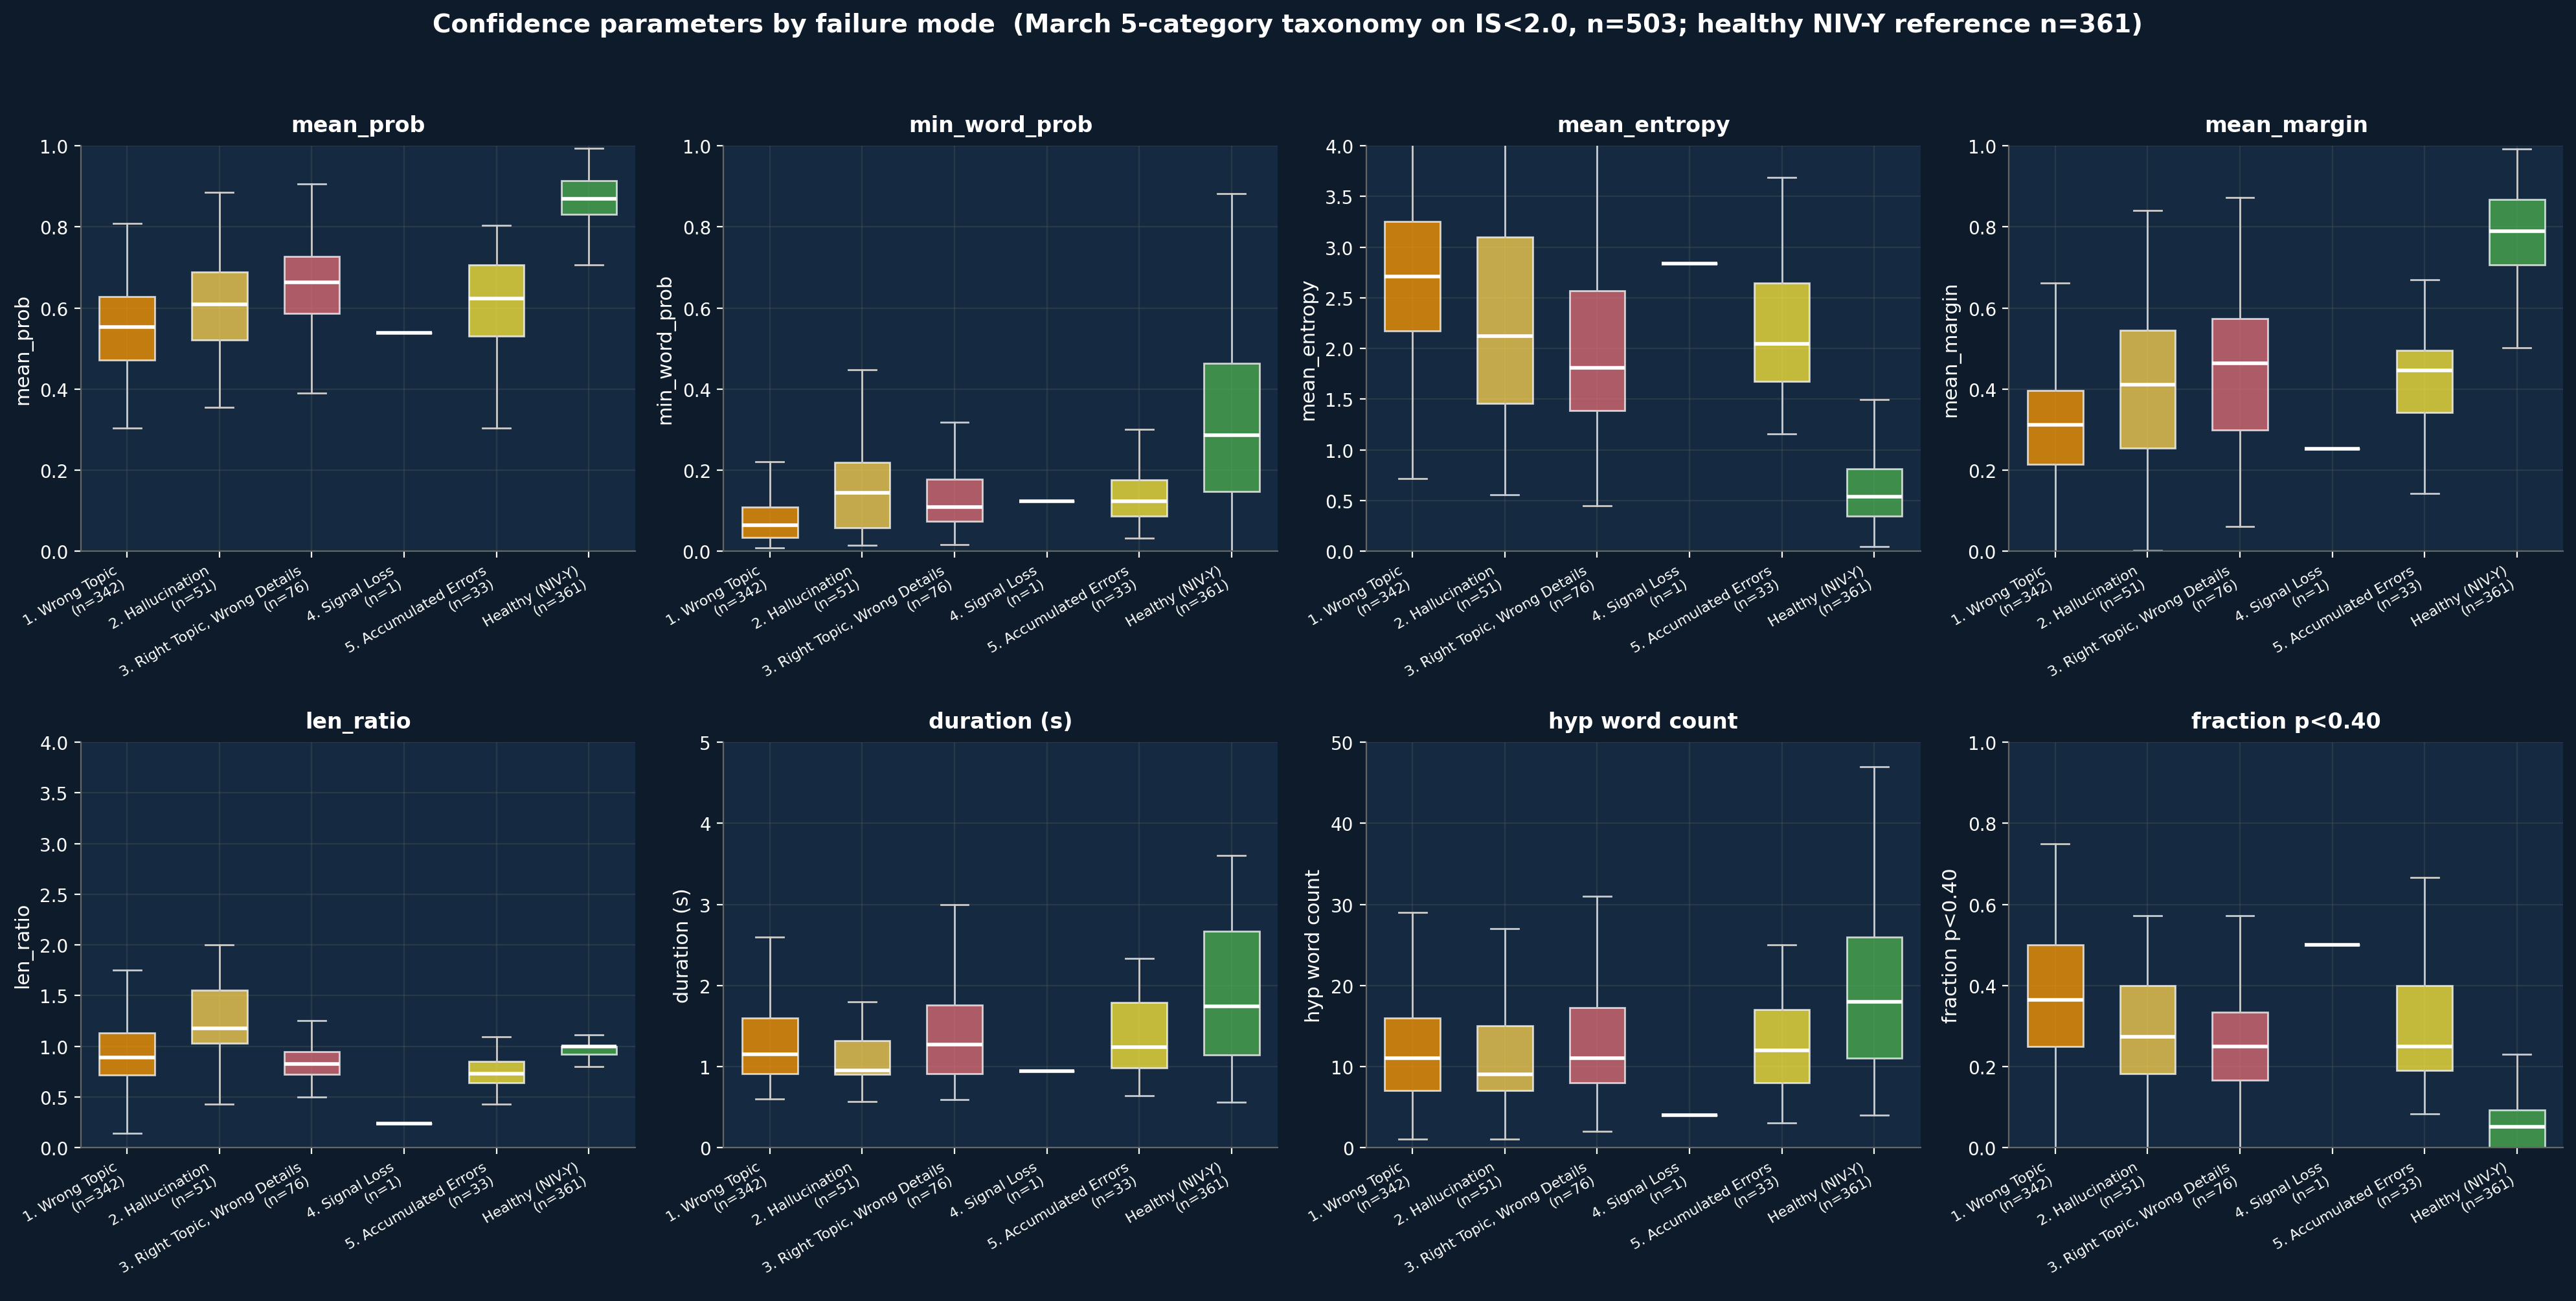
\includegraphics[width=0.95\textwidth]{conf_failure_mode_profile.png}
\caption{Boxplots of eight confidence parameters across the five March failure categories plus the healthy NIV-Y reference. Wrong Topic dominates ($\sim 68\%$) -- the model commits decisively to a wrong domain. Confidence collapses uniformly on every parameter for failures \emph{except} \texttt{mean\_prob}, where Wrong Topic still hovers in the medium band -- the deck's ``confidence color cannot detect topic substitution'' caveat.}
\end{figure}

\begin{table}[H]
\centering
\scriptsize
\begin{tabular}{lrrrrrrrr}
\toprule
\textbf{Category} & \textbf{n} & \textbf{m\_prob} & \textbf{min\_wp} & \textbf{m\_ent} & \textbf{dur (s)} & \textbf{NEA} & \textbf{WER\%} & \textbf{IS} \\
\midrule
1. Wrong Topic                & 342 & 0.55 & 0.08 & 2.74 & 1.39 & 0.7  & 137 & 1.03 \\
2. Hallucination              & 51  & 0.59 & 0.16 & 2.27 & 1.19 & 5.6  & 145 & 1.39 \\
3. Right Topic, Wrong Details & 76  & 0.65 & 0.16 & 1.97 & 1.42 & 4.4  & 71  & 1.65 \\
4. Signal Loss                & 1   & 0.54 & 0.12 & 2.84 & 0.94 & 0    & 100 & 1.91 \\
5. Accumulated Errors         & 33  & 0.62 & 0.13 & 2.14 & 1.37 & 31.5 & 51  & 1.77 \\
\midrule
\textbf{Healthy (NIV-Y)}      & 361 & \textbf{0.86} & \textbf{0.32} & \textbf{0.62} & \textbf{1.93} & \textbf{84.6} & \textbf{22} & \textbf{4.33} \\
\bottomrule
\end{tabular}
\end{table}

\subsection{Trajectory shape predicts outcome}

\begin{figure}[H]
\centering
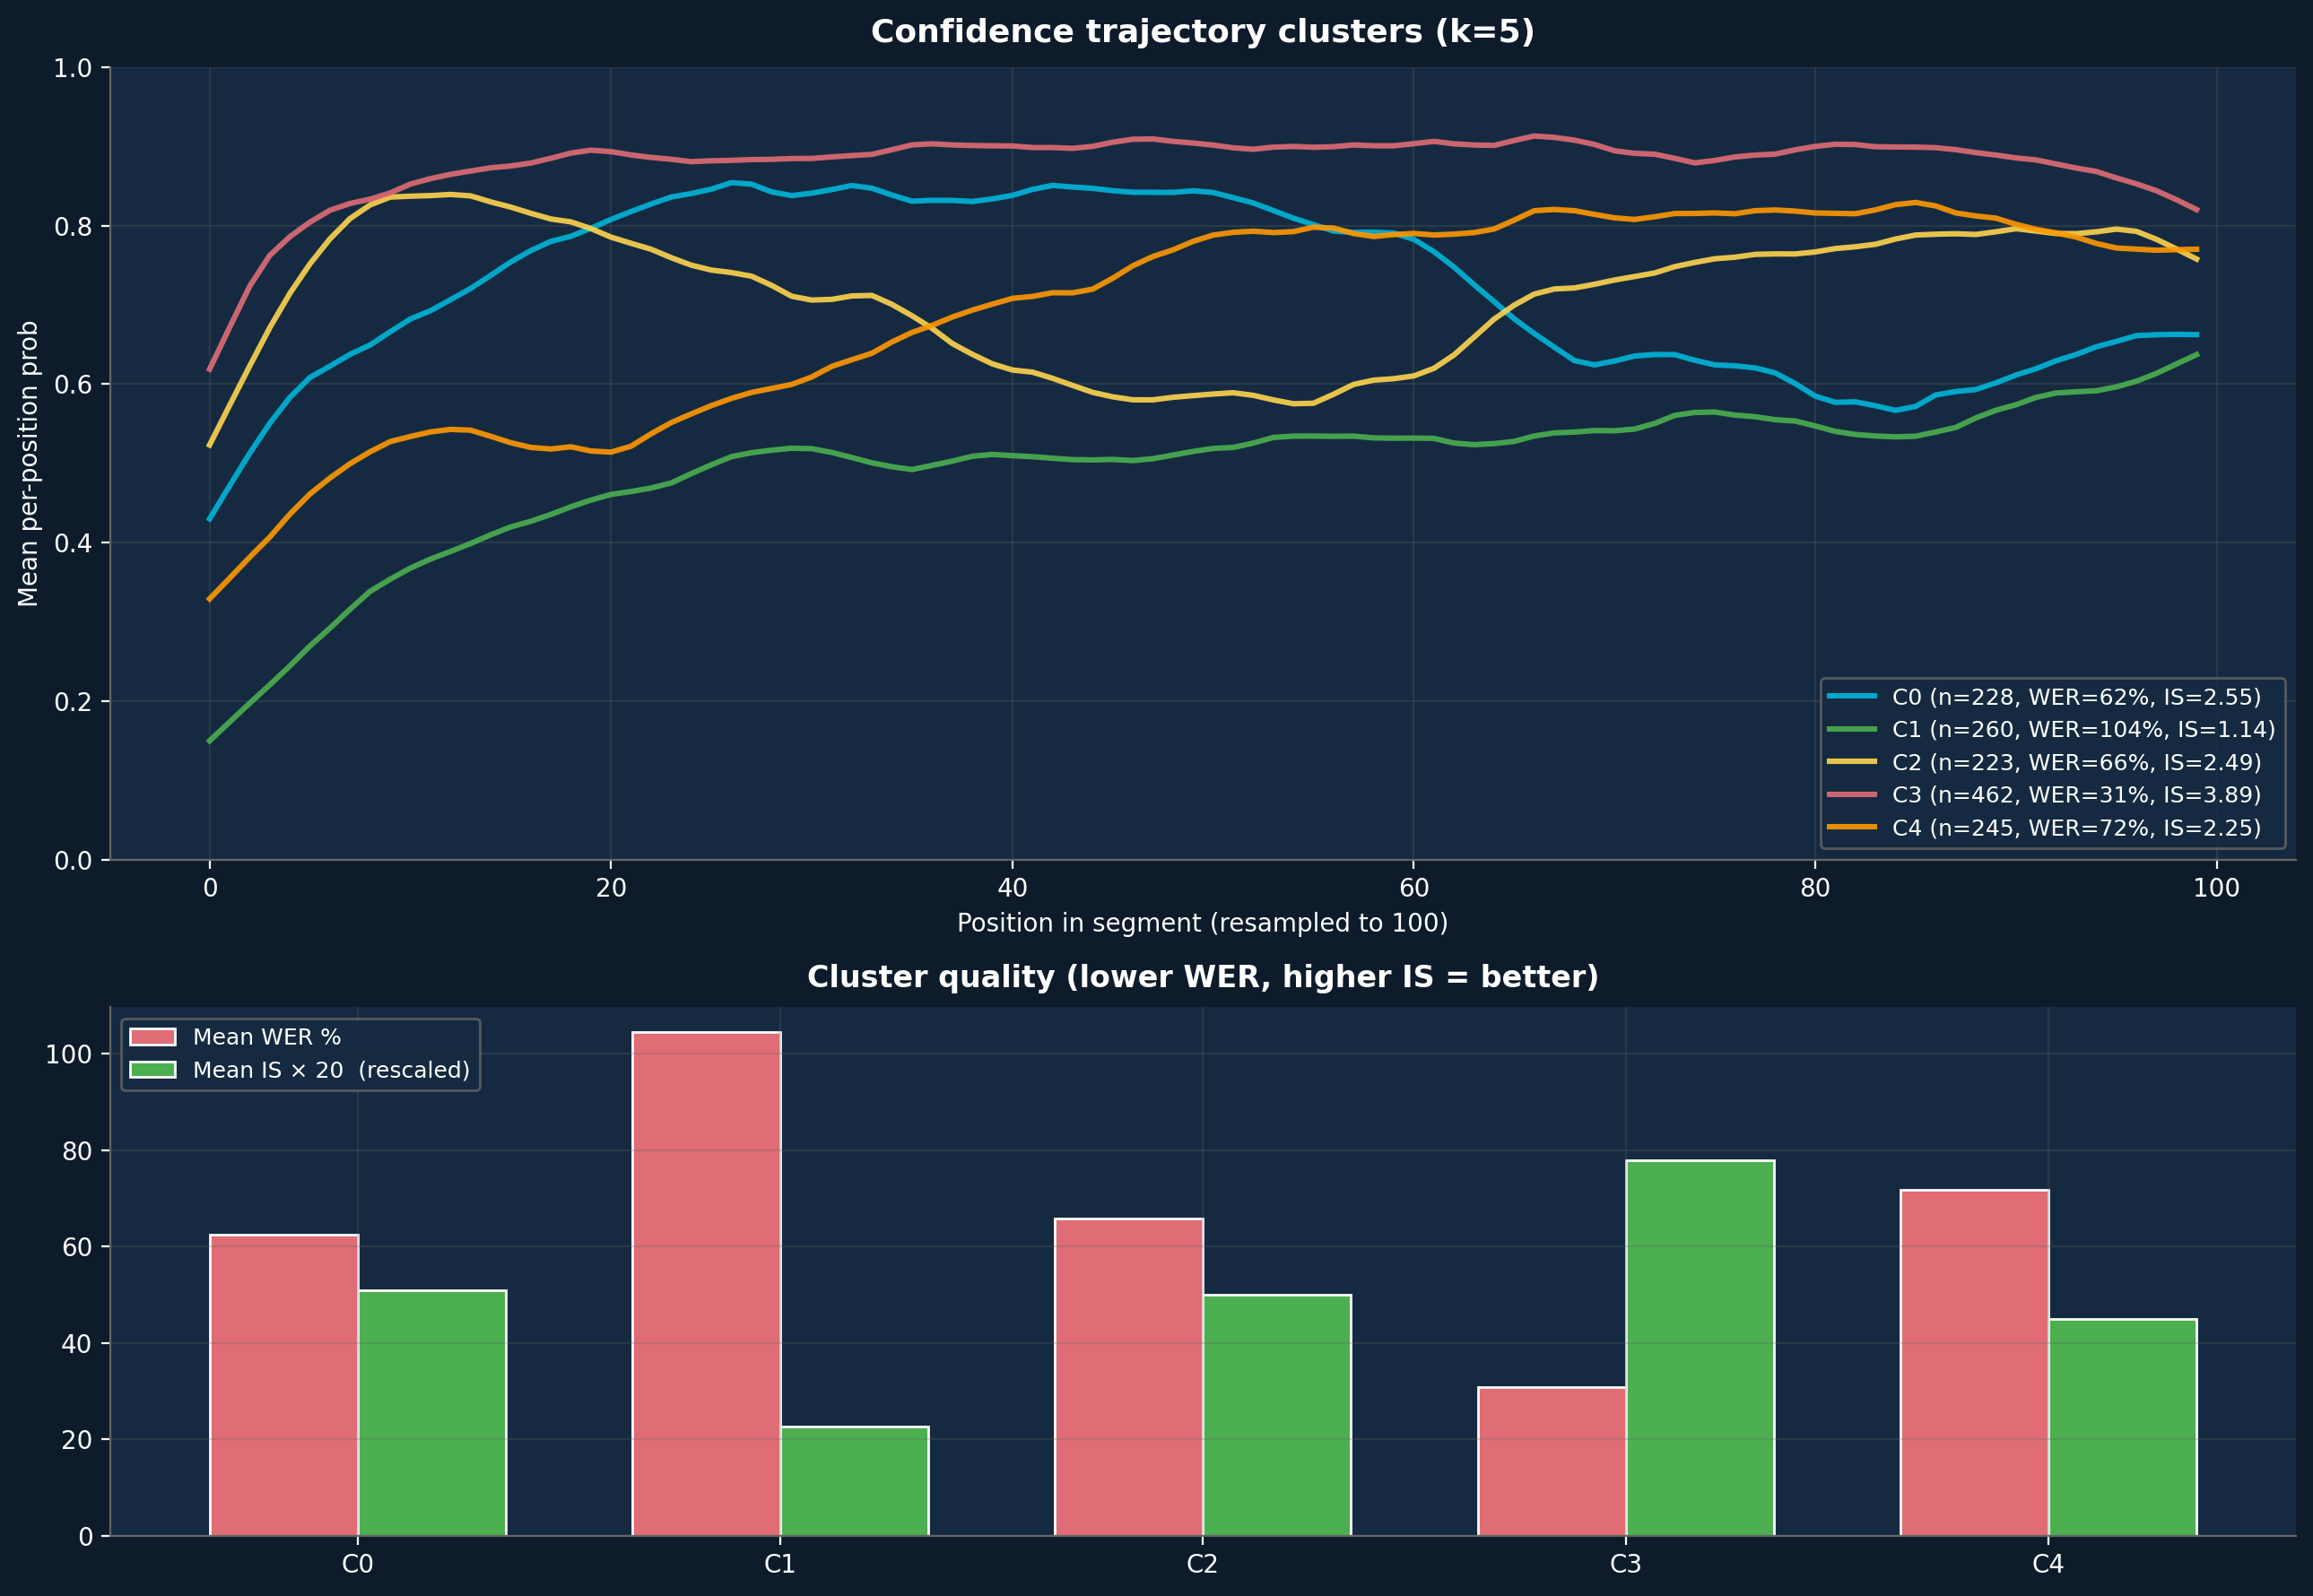
\includegraphics[width=0.92\textwidth]{conf_trajectory_clusters.png}
\caption{Top: $k=5$ cluster centroids on length-normalised per-position confidence trajectories. Bottom: per-cluster mean WER (coral) and mean IS rescaled $20\times$ (green). Flat-high cluster (C3): mean WER $\mathbf{31\%}$, IS $3.89$, $64\%$ NIV-Y. Uncertain-throughout (C1): mean WER $\mathbf{104\%}$, IS $1.14$, $\mathbf{92\%}$ NIV-N. The shape difference is visible after just a few tokens -- viable as a runtime ``give up early'' hook (Mission 11).}
\end{figure}

% ===================================================================
\section{What confidence cannot tell us, and what's next}
% ===================================================================

Confidence has three blind spots, all visible in the failure-mode breakdown:

\begin{enumerate}[leftmargin=*, itemsep=2pt, topsep=2pt]
  \item \textbf{Wrong Topic} (68\% of bad segments) -- model commits decisively to a wrong domain; \texttt{mean\_prob} sits in the medium band, no confidence signal sharp enough to flag. Needs semantic similarity (reference-required) or a topic-conditioned LM scoring the hyp for surprise relative to the source video's topic. \emph{Mission 8.}
  \item \textbf{Right Topic, Wrong Details} (15\%) -- closest of any failure mode to healthy in confidence space. Model knows the topic but loses the specific entities. Needs NEA F1 (reference-required) or beam disagreement -- if the chosen beam dropped a number that other beams kept, that's a flag. \emph{Mission 6 (all-20-beams).}
  \item \textbf{The ``billion $\to$ million'' problem} -- single high-confidence wrong content word inside an otherwise-fine segment. Bypasses all current signals because the model is decisive on the wrong answer. Needs source-context priors or visual disambiguation. \emph{Long-term.}
\end{enumerate}

\textbf{Recommendations.}

\begin{enumerate}[leftmargin=*, itemsep=2pt, topsep=2pt]
  \item Use \texttt{mean\_word\_prob} $\ge 0.80$ as the runtime quality gate. Already exposed via \texttt{make\_report.py --word-confidence} as \texttt{sentence\_confidence}.
  \item For per-word coloring display, gate the rendering on segment-level \texttt{mean\_word\_prob} $\ge 0.82$ (the band-reliability threshold from the full report). Below that, hide or banner.
  \item Mission 6 (all-20-beams capture) -- highest-leverage next-sprint item. Top-3 entropy is $r=0.95$ redundant with full entropy; we need genuine beam disagreement.
  \item Mission 8 (topic-conditioned LM for hyp rescoring) -- handles the Wrong Topic hole, 68\% of bad segments.
  \item Mission 11 (mid-decode trajectory monitoring) -- runtime ``give up early'' hook from Section 3.
\end{enumerate}

\vspace{0.3em}
\noindent\textcolor{argosGray}{\small\emph{For calibration analysis (overall ECE, stratified band reliability, three-tier display policy) and the reproduce command, see the full 17-page report at \texttt{docs/confidence/confidence\_full\_analysis.pdf}.}}

\end{document}
